\documentclass{article}
\setlength\topmargin{0pt}
\addtolength\topmargin{-\headheight}
\addtolength\topmargin{-\headsep}
\setlength\oddsidemargin{0pt}
\setlength\textwidth{\paperwidth}
\addtolength\textwidth{-2in}
\setlength\textheight{\paperheight}
\addtolength\textheight{-2in}
\usepackage{layout}
\usepackage{amsmath}
\usepackage{algorithm}
\usepackage{verbatim}
\usepackage[noend]{algpseudocode}
\usepackage{graphicx}
\graphicspath{ {./} }


\title{\vspace{-2.0cm}CS M152A Project 5 Report}
\author{Melody Chen}

\begin{document}
\maketitle
\section{Introduction and Requirement} 
The focus of this lab is for students to learn about how to design finite state machine that matches the specified behavior and to use the Xilinx ISE software to design and test state machines. Finite State Machines (FSMs) are used in many real world systems. An FSM has a finite number of states and can be in one state at a given time. There are two types of FSM machines: Moore Machine and Mealy Machine. A Moore machine's output only depends on which state it is in, but a Mealy machine's output depends on both the current state and input. \par
For this assignment, we're tasked with designing a FSM that models behavior of a parking meter which simulates coins being added and displays the appropriate time remaining. The time remaining will be displayed on a four-digit common anode seven-segment LED display that is on the Nexys3 board. The four digits is each composed of seven segments arranged in pattern shown in diagram below with LED light embedded in each segment. For example, to display the digit 0, we will pass in \texttt{Cathode[6:0] = 7'b0000001} as a vector and if we want 0 to be our least significant digit, anode 0 should be set to low, while anode 1-3 set to high. 
\begin{center}
    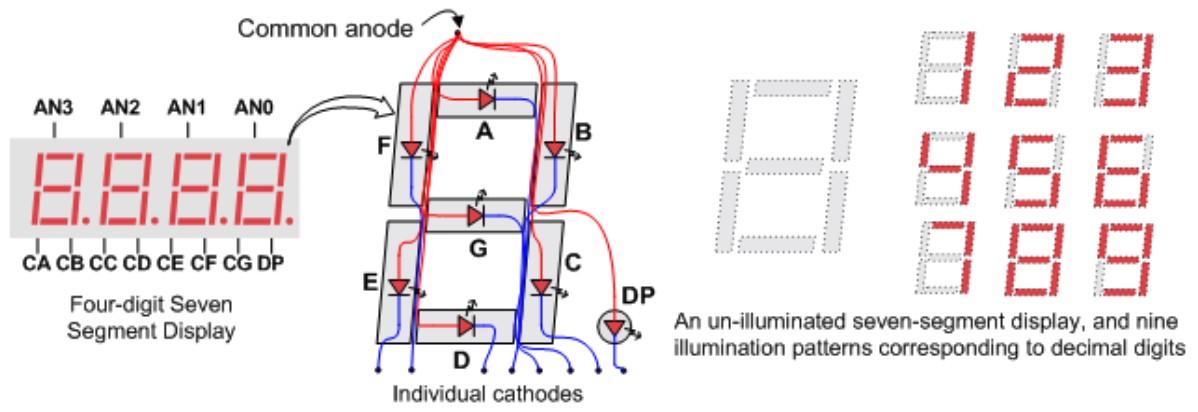
\includegraphics[scale=0.4]{7segment.png} \\
    \caption{7-segment Display Diagram from Nexys 3 Reference Manual}
\end{center} 
\noindent Our parking meter should have the following characteristics:
\begin{enumerate}
    \item Input buttons rerpesent different types of coins and 7-segment LED display will display time remaining before meter expires in seconds.
    \item When time remaining is zero, 0000 should be flashed at 1Hz with 50\% duty cycle. When time remaining is below 180, it should be flashed at 0.5Hz with 50\% duty cycle. When time remaining is above 180, there is no need to flash time remaining. 
    \item Our time remaining for parking meter cannot exceed 9999. If it does, display 9999.  
\end{enumerate}
More specifics about behavior of parking meter will be discussed in the following sections.


\section{Design Description}
For the design and implementation of the parking meter FSM, I followed guidance provided in the project specifications and consulted Project 4 Manuscript. I first consider the inputs provided and what my FSM will need to output. We want to output remaining time on parking meter via a seven-segment vector \texttt{led\_seg} and 4 one bit anode signals \texttt{a1, a2, a3, a4} given the following inputs shown in diagram below:
\begin{center}
    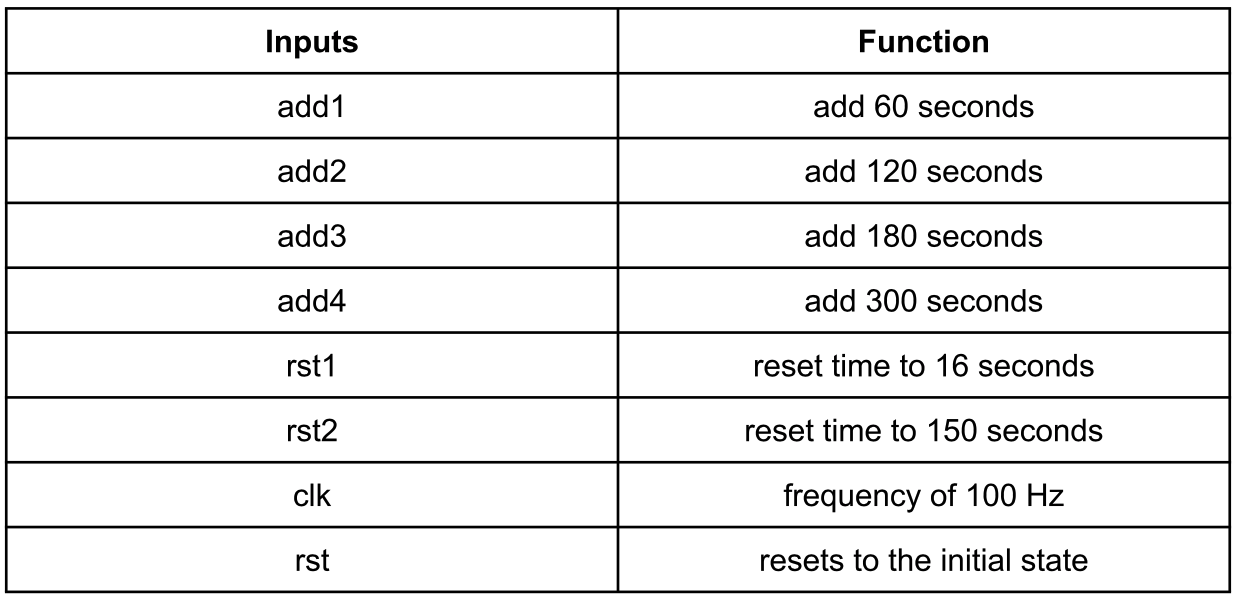
\includegraphics[scale=0.4]{inputsummary.png} \\
    \caption{Summary of Required Inputs for FSM taken from Project Manuscript}
\end{center} 
I then designed my FSM with around 8 states that correctly captures the behavior described in the manuscript. My FSM is a Moore machine, meaning that my output depends only on which state I am in, regardless of the inputs. Because it is a Moore machine, I have many states, but that is to ensure for the correct behavior for every possible combination of inputs into my FSM. 
\begin{center}
    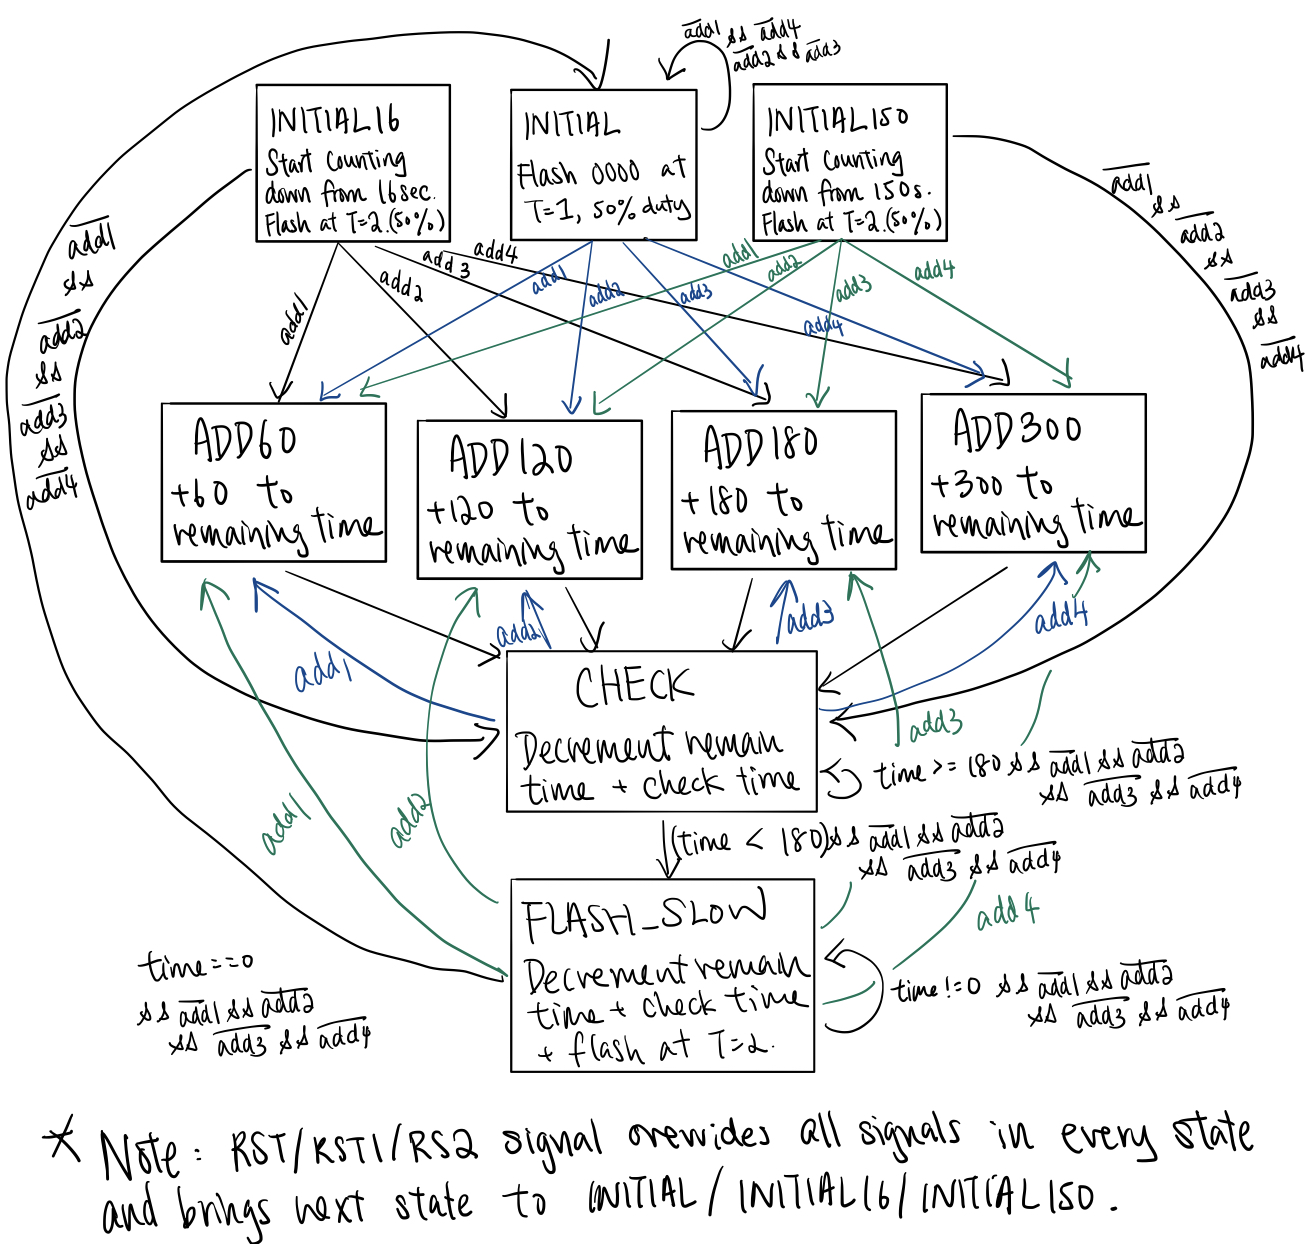
\includegraphics[scale=0.25]{FSM-diagram.jpeg} \\
    \caption{Moore FSM Design of my Parking Meter}
\end{center} 
Descriptions of states and transitions of above FSM:
\begin{itemize}
    \item Once \texttt{rst} signal is 1, we will begin at the INITIAL state, where we flash the current output \texttt{0000} at 1Hz with 50\% duty cycle. This state represents a parking meter that is out of remaining time. If we receive any coins to add time, we will transition to a different state.
    \item Two other reset signals are present in our FSM. If either \texttt{rst1} or \texttt{rst2} is high, we begin at INITIAL16/INITIAL150 state where instead of having no remaining time, we will start with either 16 seconds or 150 seconds remaining on our parking meter. Remaining time will be flashed at 0.5Hz as remaining time is non-zero and is below 180 seconds. Beginning in this state, time remaining should decrease by 1 every second. 
    \item From the three INITIAL states, if either \texttt{add1, add2, add3, add4} signal is 1, we transition to the corresponding ADD60/ADD120/ADD180/ADD300 state. The ADD states are where depending on which state, we add the specified number of seconds to our parking meter. Once this state ends, the time remaining on our meter should be updated. Note that during this state, time remaining is continued to being decremented by 1 per sec to simulate a real parking meter. Time remaining is also continued to be displayed in this state based on how it was displayed in its previous state, and added time will only show up after end of this state.
    \item From the INITIAL16/INITIAL150 states, if no add signals are asserted, we transition directly to the CHECK state. CHECK state checks whether time remaining is 0 or less than 180 in order for time remaining to be displayed in the appropriate manner. As before, time remaining is continued being decremented by 1 per sec. 
    \item From the four ADD states, once the specified time is added, we directly transition to the CHECK state. This is to make sure now that our time remaining increased, we are displaying the remaining time in the appropriate manner matching the new value. 
    \item In the CHECK state, we continue to decrement remaining time and display current time. Manner time is being displayed in this state is based on how it was being displayed in its previous state. Manner displayed will be updated after CHECK state. We use this state to check whether our new time remaining is greater or less than 180. If it is greater, we stay in this state as to continue checking if after the next second our time will be less than 180. If it is less than 180, we transition to FLASH\_SLOW state. If we receive add signal in this state, we directly transition to the corresponding ADD state.
    \item In FLASH\_SLOW state, time is continue being decremented and it is displayed at 0.5Hz with 50\% duty cycle as time is below 180 seconds. If we receive add signal in this state, we directly transition to the corresponding ADD state to make sure time is increased. Otherwise, if time left is zero, we transition back to INITIAL for 0000 to be flashed at 1Hz. If time left is greater than zero and no add signal received, we stay in this state to continue decrementing and displaying time. 
    \item Note 1: If \texttt{rst = 1} or \texttt{rst1 = 1} or \texttt{rst2 = 1}  at any point in our state diagram, it overrides other signal and arrows, and we directly return to the corresponding INITIAL/INITIAL16/INITIAL150 state.
    \item Note 2: Time remaining is \textbf{always} being decremented by 1 every second if it is not zero(i.e. we're not in the INITIAL state). Time remaining is \textbf{always} being displayed, but there could be a 1-2 cycle delay as it takes time for our FSM to process input signal and update the outputs. 
\end{itemize}
To implement the above FSM in Verilog, I created the \texttt{parking\_meter} top module that takes in input listed in the table above and outputs: 4 anode signals, vector \texttt{led\_seg}, and time remaining in 4 BCD digits. Within my module, I initialized parameters representing all the states I have with a unique 4 bit binary number, two 4-bit registers \texttt{current\_state} and \texttt{next\_state}, a \texttt{time\_left} register to keep track of number of seconds remaining in decimal, and various internal signals and counters for keeping track of time. I have 4 main always block each with a specific task:
\begin{enumerate}
    \item Sequential always block to update \texttt{current\_state} to \texttt{next\_state} at every \texttt{posedge} of the clock or update \texttt{current\_state} to INITIAL/16/150 state when either \texttt{rst, rst1, rst2 = 1}.
    \item Combinational always block to decide what \texttt{next\_state} should be based on the current state and current inputs.
    \item Sequential always block to determine how much \texttt{time\_left} based on the current state and internal counters that exploit the input clock to keep track of time.
    \item Sequential always block to determine the 4 1-bit anode signals and vector \texttt{led\_seg}, which both control what is shown on our 7-segment LED display, based on our current state, internal counters, and our \texttt{time\_left} register.
\end{enumerate}
Aside from the blocks mentioned above, I also have smaller combinational logic blocks to determine value of \texttt{led\_seg} based on time remaining. I also have smaller sequential logic blocks that control my internal counters that produces signal to inform other blocks when to decrement \texttt{time\_left} register(i.e. when 1 second has passed) and signal for the appropriate flashing of our display. The logic and design of these counters are heavily based on previous projects such as 4-bit counter and clock divider.
\begin{center}
    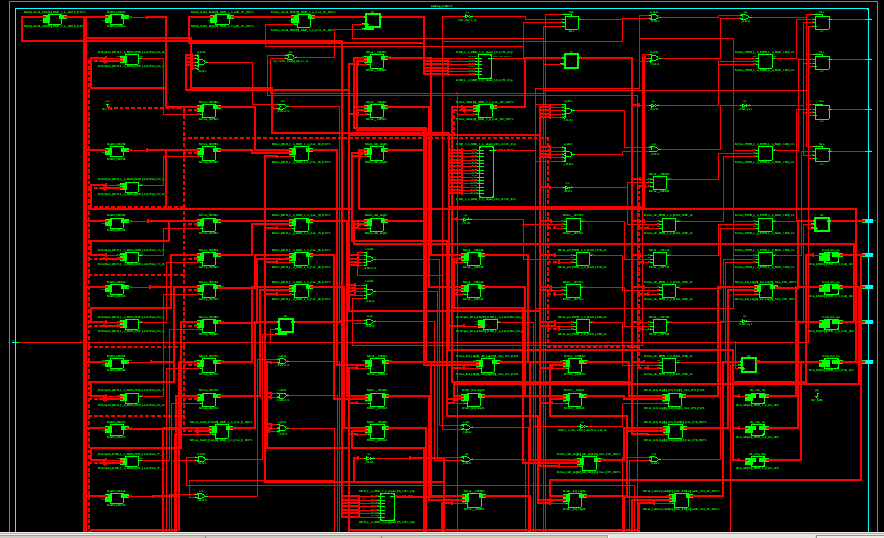
\includegraphics[scale=0.4]{rtl-lab5.png} \\
    \caption{RTL Schematic of Parking Meter FSM}
\end{center} 
From first look, the RTL schematic above looks a bit complicated and filled with registers, muxes, and counters. This makes sense as our FSM is fairly complicated having to keep track of internal counters, over 4 always blocks with layers of conditions in addition to combinational logic for determining next state and to produce signals for 7-segment display. My Verilog code results in this schematic being generated(layers of mux, gates for combinational logic, and many registers) as the logic for determining what the remaining time is based on input signals on top of how to display the remaining time based on current time needs to be implemented through series of mux logic, registers/D-Flipflops are essential for our internal counters, and gates for our combinational logic.
\section{Simulation Documentation}
To test whether the FSM I implemented works as the manuscript described, I created my testbench that tests not only all the possible types of inputs, but all of the possible special cases, such as adding signal received at the exact time time is decremented. I provided a 100Hz clock input clock in my testbench as specified by the manuscript.  To simulate behavior of someone interacting with the parking meter, in my testbench, I at each positive edge of the input clock, I change a particular input to observe how my FSM will deal with the change in input or I don't change any input to observe my FSM counting down. Below are all the different cases I tested and their respective waveform. \par
\noindent Note that in all the simulation waveforms shown below in addition to the outputs mention in the previous sections, I show an additional two outputs \texttt{time\_left}, decimal representation of how much time remains, and \texttt{current\_state}, binary representation of our current state, to illustrate how my FSM operate and for ease of readability. In addition, signals in waveforms are color coded: light blue indicates the two outputs I added, pink indicates output specified by manuscript, and green indicates inputs provided to FSM.
\begin{enumerate}
    \item \textbf{Transition from No Time Remaining to 60 sec with \texttt{add1} signal} \\
    This case represents a parking meter that is not being used and has no time remaining, and then someone parks a car and added 60 seconds to the meter through the \texttt{add1} signal. How I tested this case was to first set \texttt{rst} to high for one clock cycle to put parking meter at INITIAL(0000) state. Then, after almost one second, I set the \texttt{add1} signal to high for one clock cycle to simulate someone putting coins in to the meter and then I continued flipping clock signal to observe its behavior. We can observe from the waveform below that while there is no time remaining in our meter, outputs \texttt{val1-4} remain zero which is the correct behavior. The \texttt{led\_seg} vector has value \texttt{0000001} which is correct vector for outputting 0 on a 7-segment display. We also observe outputs \texttt{a1-4} rotating which of the four signal is low in order to display 0 on all four 7-segment displays. Right after \texttt{add1} signal is high for 1 cycle, we immediately observe \texttt{time\_left} increased from 0 to 60 seconds as expected. After 1 sec, we see that value of \texttt{led\_seg} changes and alternates between vector for digit 0 and 6 as expected. 
    \begin{center}
        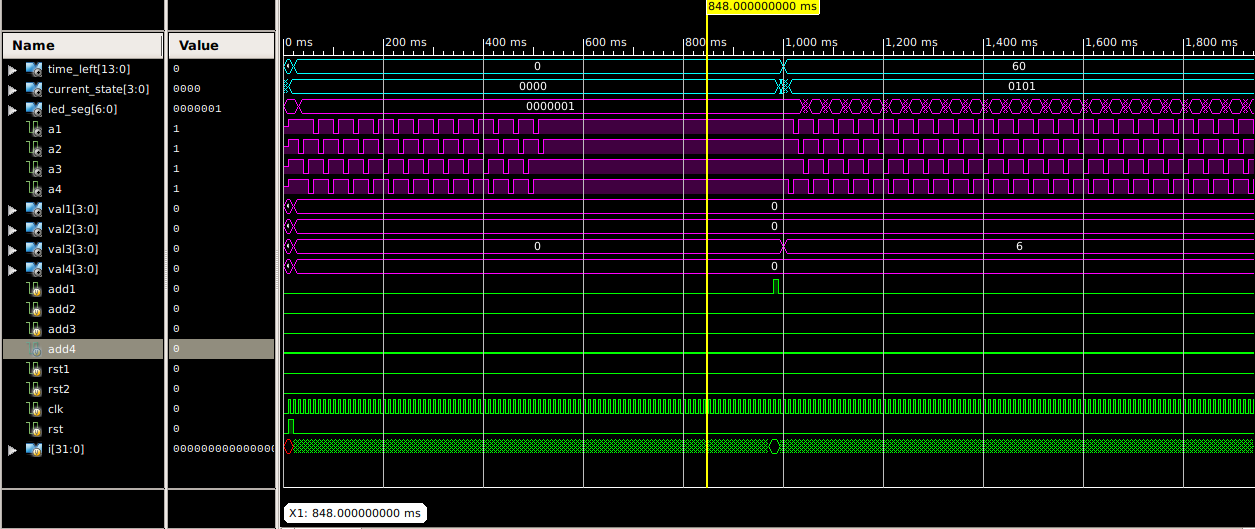
\includegraphics[scale=0.36]{waveform-1.png} \\
        \caption{Simulation Waveform for Case 1}
    \end{center}
    \par
    
    \item \textbf{Correct Flashing of Time Remaining under 180 sec}\\
    This case represents a time meter that has less than 180 seconds remaining where time is decreasing appropriately and flashed at period of 2 seconds. To test this case, I simply continue to flip the clock signal for a 100Hz clock for a specific number of cycles. From the diagram below, in addition to \texttt{time\_left} being decremented exactly after every 1 second and the correct \texttt{val-4} values, we also observe only when time remaining is an odd number, all \texttt{a1-3} remain high meaning nothing is shown on the displays. This is correct behavior as to have a period of 2 seconds with 50\% duty cycle, we only want there to be time remaining shown for 1 second. The specs specified only the even times to be shown. 
    \begin{center}
        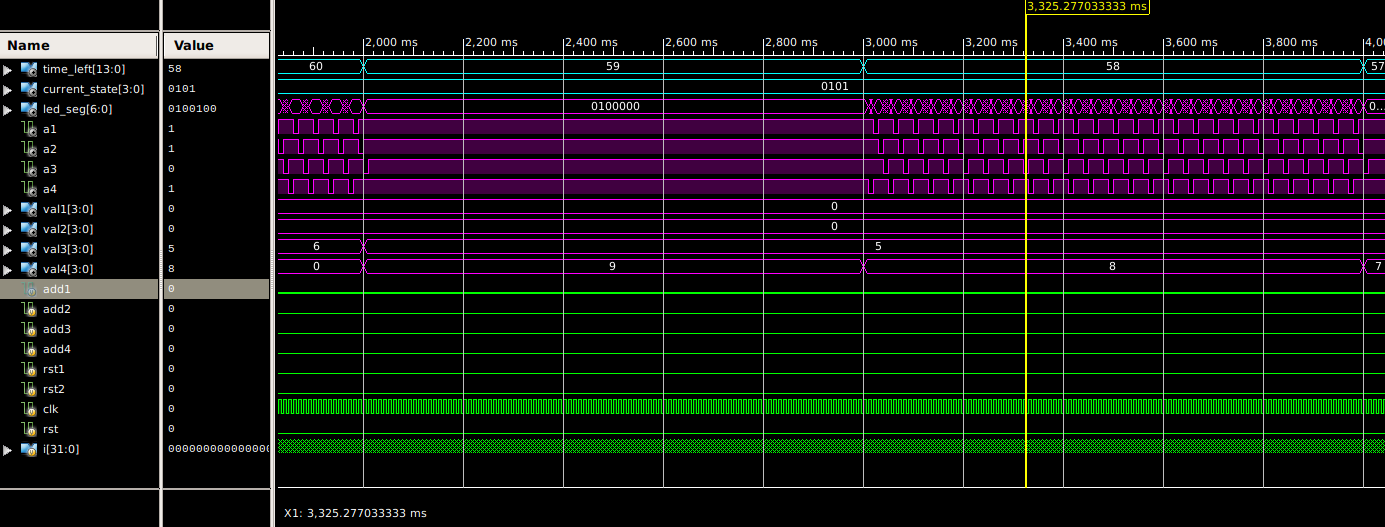
\includegraphics[scale=0.34]{waveform-2.png} \\
        \caption{Simulation Waveform for Case 2}
    \end{center}  \par

    \item \textbf{Adding time with \texttt{add2} signal while time remaining is under 180 sec}\\
   This case represents someone adding 120 seconds to a parking meter that has current remaining time less than 180 seconds. To simulate this behavior, I set the \texttt{add2} signal to high for one clock cycle while time remaining is displaying 57 seconds. From the diagram below we can see that at 4000ms we go from 58 sec to 57 sec remaining. At around 4200ms, our FSM detects the \texttt{add2} signal and time remaining becomes 177 sec. Since \texttt{add2} signal is detected around 200ms after our FSM has been showing 57sec, we expect 177 sec to be displayed not for a full 1 second, but only for the remaining 800ms. This is because we don't want our parking meter to "gain extra time" just because coin is inserted when 56.8 seconds remain instead of 57 seconds. This matches the behavior of our FSM as at exactly 5000ms, 1000ms after time remaining decremented to 57 seconds, 177 sec is decremented to 176 seconds. No extra time is gained. 
    \begin{center}
        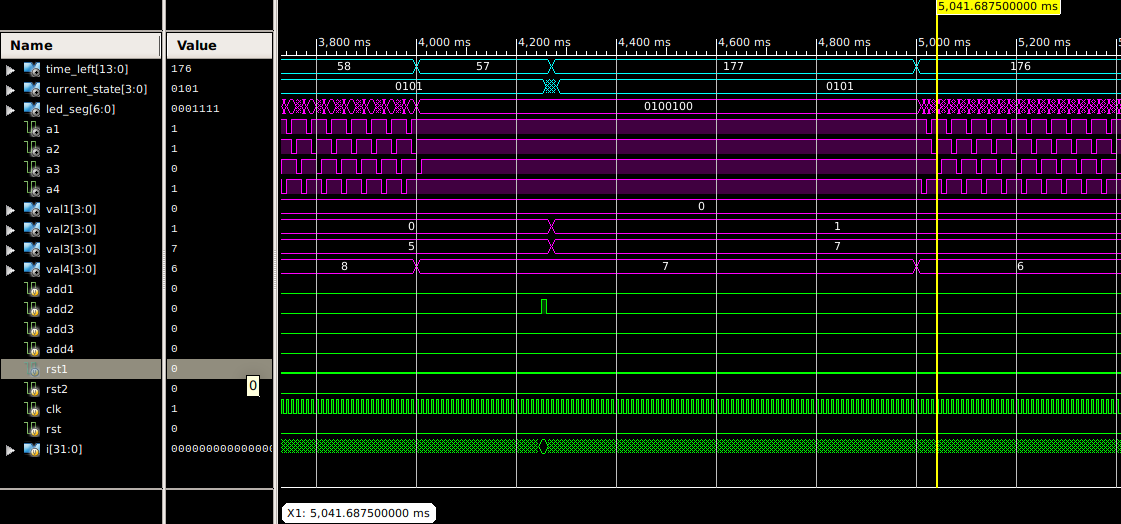
\includegraphics[scale=0.37]{waveform-3.png} \\
        \caption{Simulation Waveform for Case 3}
    \end{center}
    \par
    
    \item \textbf{Adding time with \texttt{add3} signal with resulting time exceeding 180 sec}  \\
    This case represents when parking meter has time remaining below 180 seconds and someone put in coins to add 180 seconds of time. To simulate this behavior, I set the \texttt{add3} signal to be high for one clock cycle while time remaining is displaying 174 seconds. As mentioned in the last case, since signal is detected midway through display of 174 sec, we only want 354 sec to be shown for the remaining half of the second(and decrement right after) instead of for a full second. We can observe this correct behavior in our waveform below where 180 seconds is correctly added and at exact 8000ms, 354 is decremented to 353. We can also observe from our \texttt{a1-4} signals that our 7-segment display is no longer being flashed at 0.5Hz, but continued to be displayed without being flashed. This matches behavior in the manuscript.
    \begin{center}
        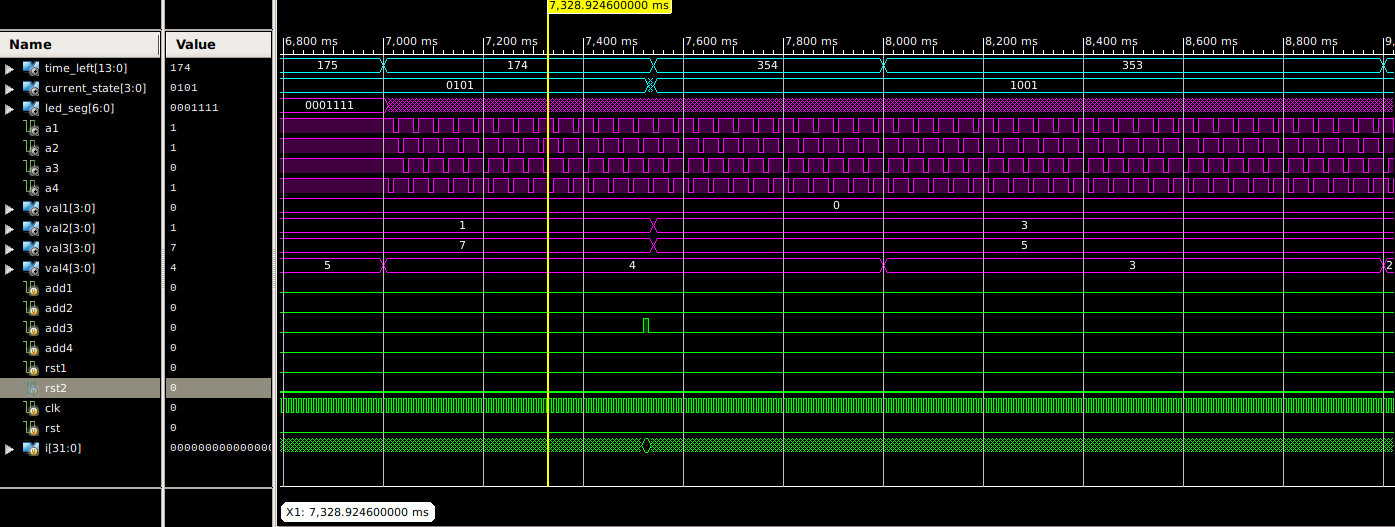
\includegraphics[scale=0.30]{waveform-4.png} \\
        \caption{Simulation Waveform for Case 4}
    \end{center}

    \item \textbf{Adding time with \texttt{add4} signal while time remaining exceed 180 sec}  \\
    This case represents when parking meter has time remaining that is above 180 seconds and someone put in coins to add 300 seconds of time. To simulate this behavior, I set the \texttt{add4} signal to be high for one clock cycle while time remaining is displaying 351 seconds. As mentioned in the last case, since add signal is detected around 800ms after time remaining began displaying 351, we only want 651 sec to be shown for 200ms instead of for a full second. We can observe this correct behavior in our waveform below where 300 seconds is correctly added and at exact 11000ms, 651 is decremented to 650. We can also observe from our \texttt{a1-4} signals that our 7-segment display is not being flashed. This matches behavior in the manuscript.
    \begin{center}
        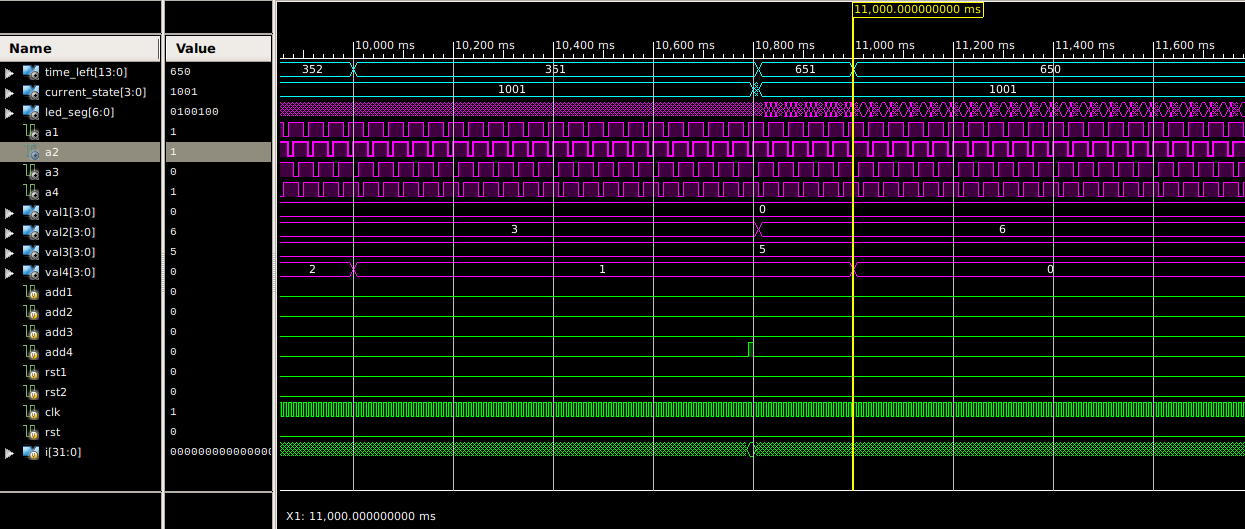
\includegraphics[scale=0.34]{waveform-5.png} \\
        \caption{Simulation Waveform for Case 5}
    \end{center}
    
    \item \textbf{Correct 7-Segment Signal for Multiplexed Display with Large Time Remaining}   \\
    In this case, we look closer into how we're producing signals for the multiplexed display and whether they will allow our 4 7-segment displays to correctly show the remaining time on our parking meter. From the waveform diagram below, we observe that current time remaining is 649 seconds. At $t=12,340s$, signal \texttt{a1} is low for 1 cycle while signals \texttt{a2-4} are high. This means that whatever is in the \texttt{led\_seg} vector is what will be displayed for the left-most digit on our display. At $t=12,340s$, \texttt{led\_seg} vector has values corresponding to showing a 0 which is correct as left-most digit of 649 is 0. At $t=12,3450s$ the next clock cycle, only anode signal that is low is \texttt{a2}, so we will display the number 6 on second left-digit of our display, which is correct. In the same manner, digit 4 will be displayed for the 3rd left-most digit and digit 9 will be displayed for the right most digit in the following cycle. Thus, our parking meter FSM correctly displays time remaining on our 7-segment displays. 
    \begin{center}
        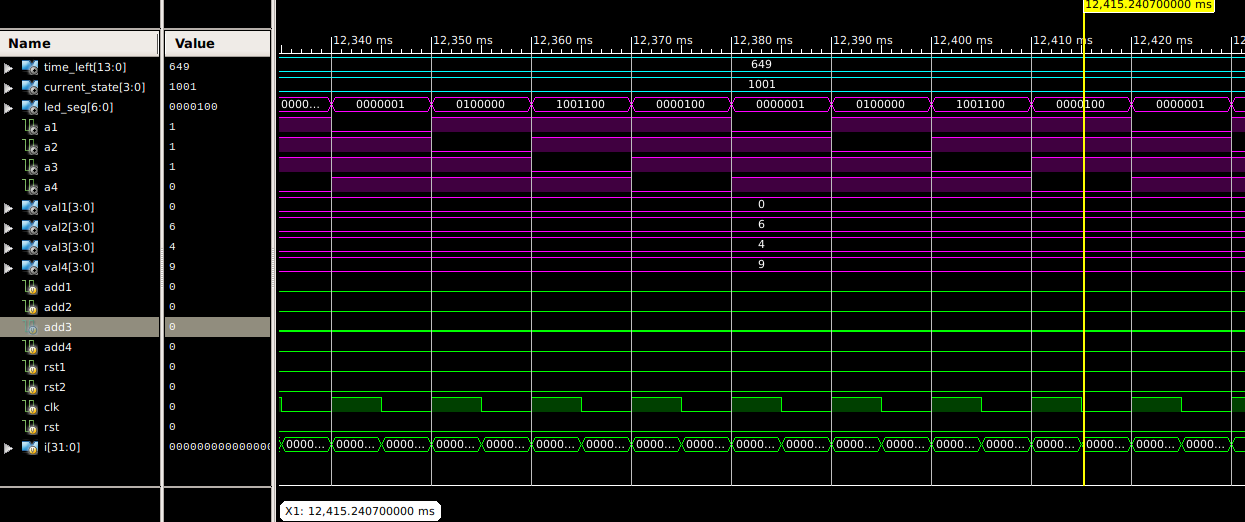
\includegraphics[scale=0.35]{waveform-6.png} \\
        \caption{Simulation Waveform for Case 6}
    \end{center}
    
    \item \textbf{Closer look at \texttt{rst1} signal when time remaining is large}   \\
    This case represents situation where our parking meter is resetted to 16 seconds remaining. As you can observe from waveform below, \texttt{rst1} is high for one cycle, and in the following cycle our time remaining is updated to 16. However, looking at the \texttt{led\_seg} value, in the cycle after reset signal is asserted, there is one cycle where we display 6 in our second left-most digit. But after that cycle, values corresponding to 16 sec is displayed. This is the correct behavior as it takes one state for our FSM to process the reset signal and compute through combination logic what should be passed to \texttt{led\_seg}. This will not affect customers of our parking meter as this occurs only for one brief cycle. We can also observe how for the rest of the cycles with time remaining being 16, the outputs are all valid.
    \begin{center}
        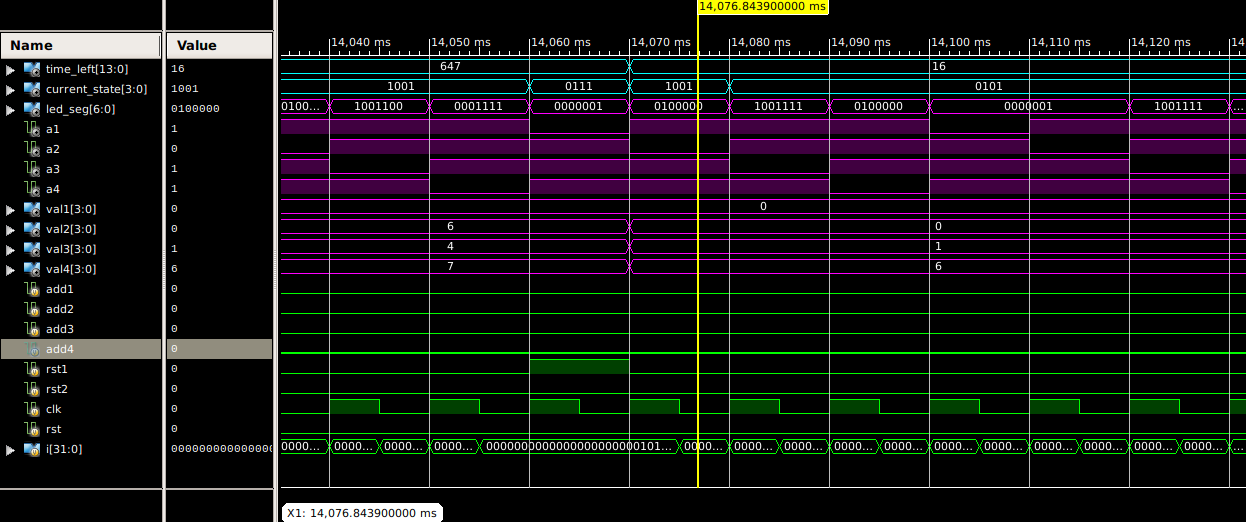
\includegraphics[scale=0.35]{waveform-7.png} \\
        \caption{Simulation Waveform for Case 7}
    \end{center}
    \item \textbf{Correct timing after reset signal while time remain decreases} \\ \\
    This case examines whether after a \texttt{rst1/2} signal, our parking meter correctly shows the time remaining from either 16/150 seconds for 1 full second. From the waveform below, we can observe that \texttt{rst1} signal is detected at $t=14070s$. So the value 16 should be displayed on our parking meter until $t=15070s$. This correctly matches what is shown in diagram below. 
    \begin{center}
        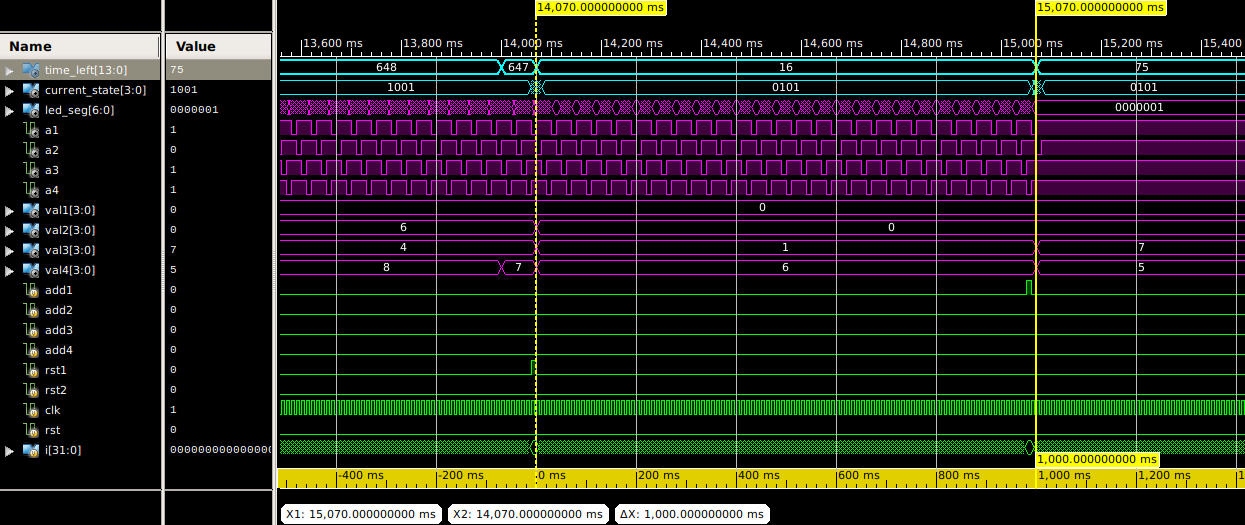
\includegraphics[scale=0.35]{waveform-8.png} \\
        \caption{Simulation Waveform for Case 8}
    \end{center}
    \item \textbf{Add signal detected right as even time is decremented to odd time} \\ \\
    This case is an edge case where right when time remaining is supposed to go down by 1, we add time into our parking meter. To simulate this behavior, I set \texttt{add1} signal to be high for one cycle when 16 second is almost decremented to 15 seconds. Without this signal, in the next cycle we were supposed to show 15, but now we should show 75 seconds remaining. 76 seconds remaining is an incorrect output as 60 seconds is added when 16 seconds becomes 15 seconds. From waveform below, we can see that our FSM correctly displays 75 seconds remaining after the \texttt{add1} signal. 
    \begin{center}
        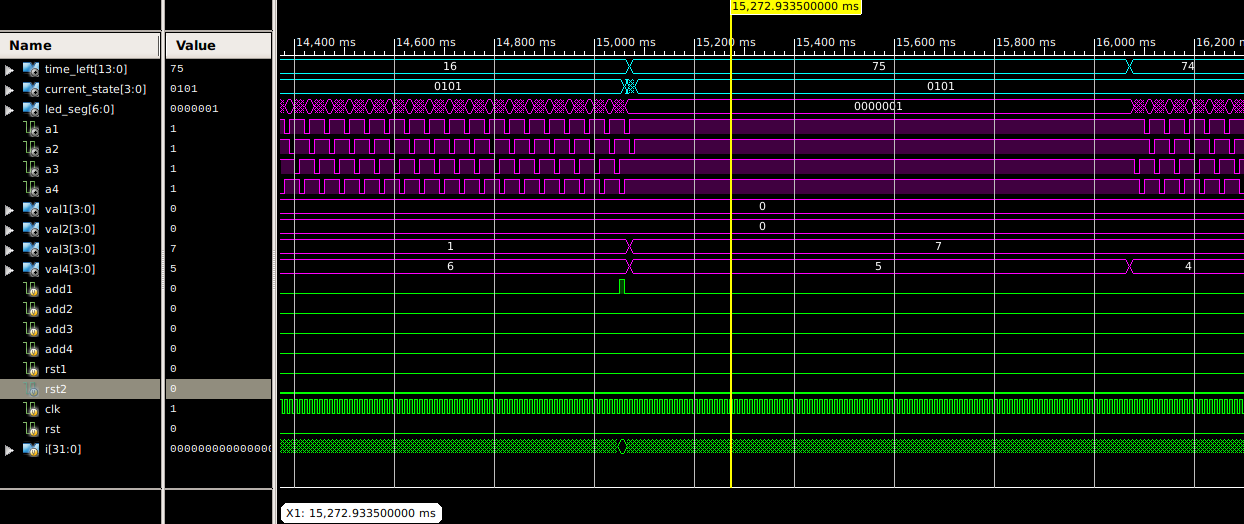
\includegraphics[scale=0.35]{waveform-9.png} \\
        \caption{Simulation Waveform for Case 9}
    \end{center}
    
    \item \textbf{Correct behavior of \texttt{rst2} signal} \\ \\
    In this case, we model the behavior of our parking meter being reset to have 150 seconds remaining. I tested this by setting the \texttt{rst2} signal to high for one cycle. From the diagram below, we can observe that FSM is correctly reset to 150 seconds at $t=17s$, at displays 150 until $t=17s$ which is the expected behavior.
    \begin{center}
        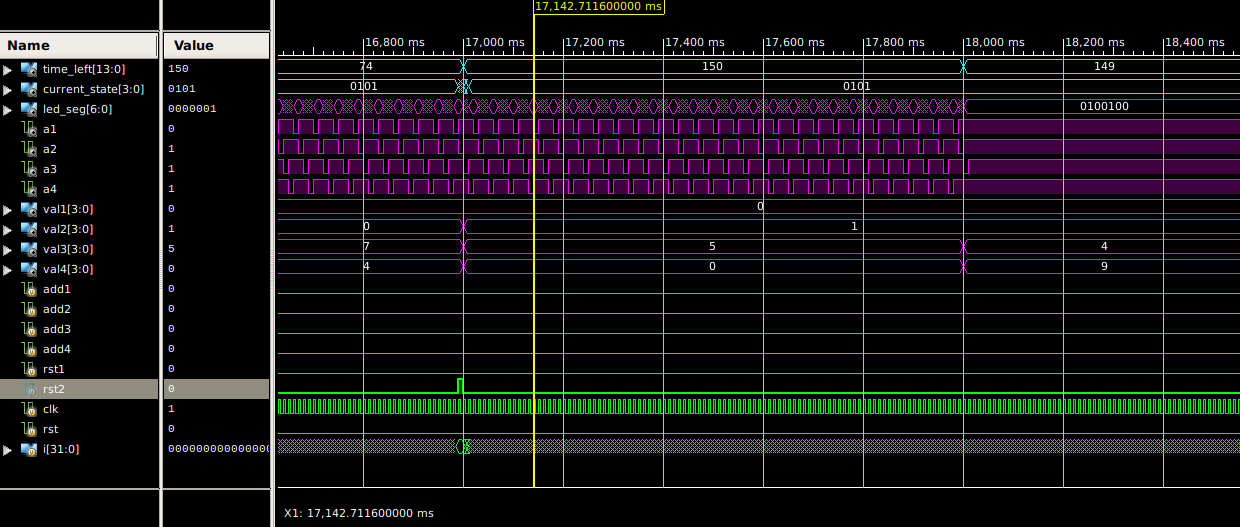
\includegraphics[scale=0.35]{waveform-10.png} \\
        \caption{Simulation Waveform for Case 10}
    \end{center}
    \item \textbf{Correct flashing of no time remaining} \\ \\
    In this case, we test whether our FSM correctly flashes 0000 at 1Hz when there is no time remaining. I tested this by simply resetting the FSM and observing its behavior as clock signal is being flipped. From the diagram below, we can observe that from $t=19.5s$ to $t=20s$, we're showing 0000 on our display, but from around $t=20s$ to $t=20.5s$, we're not showing anything on our display. This pattern continues which indicates that we're correctly displaying 0000 at 1Hz with 50\% duty cycle.
    \begin{center}
        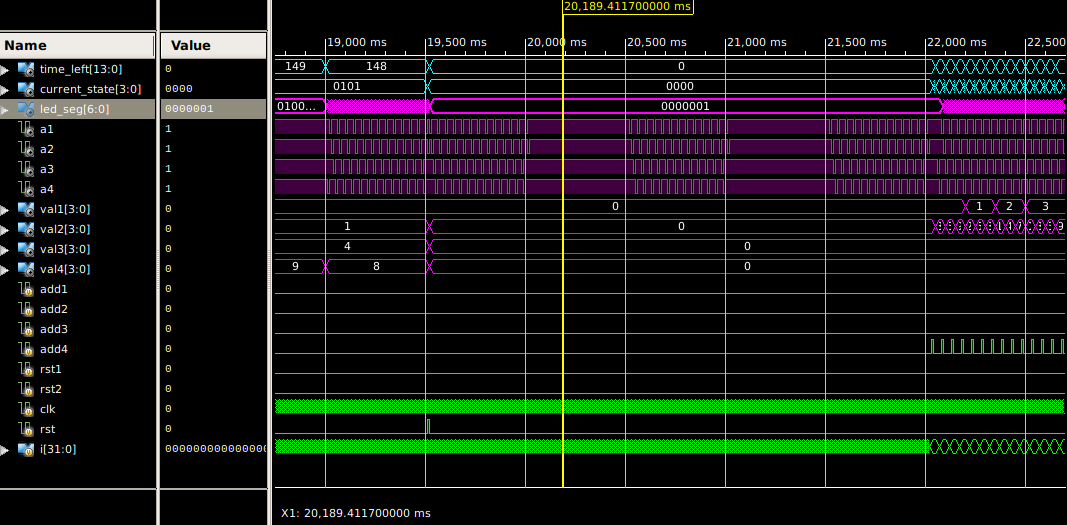
\includegraphics[scale=0.4]{waveform-11.png} \\
        \caption{Simulation Waveform for Case 11}
    \end{center}
    \item \textbf{Incrementing time remaining beyond 9999} \\ \\
    In this case, we test whether our FSM correctly behaves when we attempt to increment time beyond 9999 seconds. The expected behavior is to remain at 9999 seconds when more time is added to 9999 seconds. To test this case, I used the \texttt{add4} signal to continue to add 300 seconds to our time remaining until we reached 9999 seconds. From the diagram below, we can observe that once we attempt to add 300 seconds to 9899 seconds, we get output of 9999 seconds. This matches the behavior specified in the manuscript.
    \begin{center}
        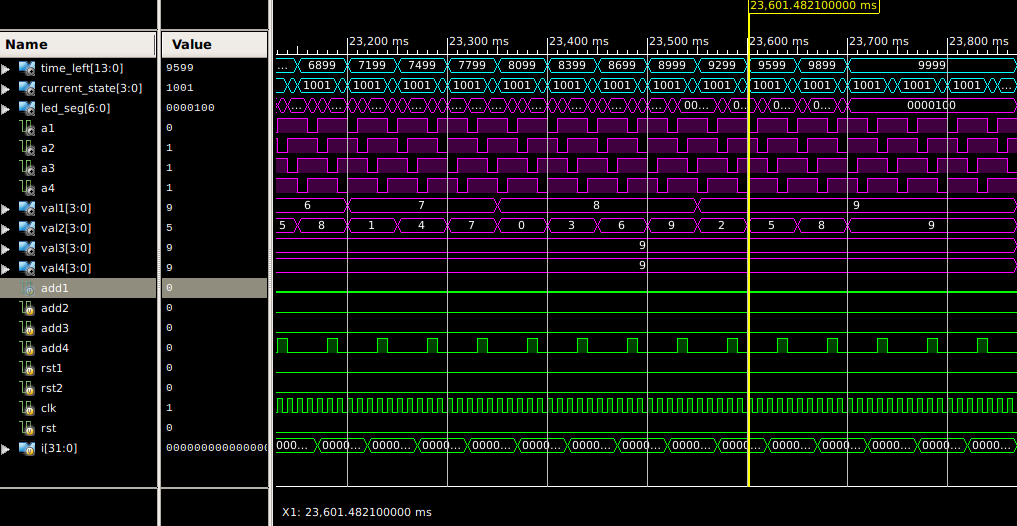
\includegraphics[scale=0.4]{waveform-12.png} \\
        \caption{Simulation Waveform for Case 12}
    \end{center}
\end{enumerate}
One bug I found during simulation for this project was that I accidentally flipped my anode signals. To have the \texttt{led\_seg} display show on the left-most bit, \texttt{a1} should be set to low while rest of anodes set to high. But I had \texttt{a1} set to high while rest of anodes set to low. Because of the simulations, I was able to quickly find this major bug and fix my FSM accordingly. 

\section{Synthesis and Implementation Report}
Sections of Synthesis and Implementation Report is attached at end of report.  From the 'Design Summary' part of the synthesis report, we can conclude the different components that my implementation of the Parking Meter FSM uses. For example, we can see that we indeed do use a lot of registers from the synthesis report and we can also see the different clock signals needed for our module. From implementation report, we can see that there is no errors when trying to implement our module, but there are a few warnings due to truncation of numbers into registers. The warnings can be ignored as in my code I made sure that truncation will definitely not occur for those registers through conditions.

\section{Conclusion} 
In this project, I designed and implemented the Parking Meter FSM according to the behavior in the project manuscript and how a real world Parking Meter will work. I designed the Parking Meter based on a Moore Machine, that has similar structure to the Vending Machine FSM implemented to in the last project. To correctly implement this, I had to first draw the FSM diagram to allow me to clearly see what output should be in each state and how to transition to a different state. One of the major difficulty I encountered in this assignment was understanding how to use the 7-segment display to display my remaining time correctly. Another major difficulty was to implement the various internal counters needed for different flashing frequencies. I was able to figure out what to do from help from my TA and from the work I did with counters and clock dividers in the previous projects. 

\newpage
\small
\section{Reports}
\subsection{Synthesis Report}
\verbatiminput{syn-report-lab5.txt}
\newpage
\subsection{Implementation Report}
\verbatiminput{imp-report-lab5.txt}

\end{document}